\chapter{Unifying Reactive Collision Avoidance and Control Allocation}
\label{chap:collision_avoidance}

To enable autonomous vehicles to operate in cluttered and unpredictable environments with numerous obstacles, such vehicles need a collision avoidance system that can react to and handle sudden changes in the environment.
This chapter discusses an optimization-based reactive collision avoidance system that uses control barrier functions integrated into the control allocation.
%We demonstrate the ability of the method to track the reference waypoints while maintaining safe distances through numerical simulations where the method is applied to autonomous surface vehicles.
We demonstrate the effectiveness of this method through numerical simulations of autonomous surface vehicles. The simulated vehicles track their reference waypoints while maintaining safe distances.
The proposed method can be readily implemented on vehicles that already use an optimization-based control allocation method.
The contents of this chapter are based on \cite{matous_unifying_2021}.

%%%%%%%%%%%%%%%%%%%%%%%%%%%%%%%%%%%%%%%%%%%%%%%%%%%%%%%%%%%%%%%%%%%%%%%%%%%%%%%%
\section{Introduction}
%Overactuated vehicles, \emph{i.e.,} vehicles with more actuators than degrees of freedom (DOFs), often use control allocation in their lowest-level controller \cite{johansen_control_2013}.
In this chapter, we consider overactuated vehicles, \emph{i.e.,} vehicles with more actuators than \acrfullpl{dof}, with a control system consisting of blocks shown in Figure \ref{fig:ccta_diagram}.
The control system contains a long-term, deliberate planner, a high-level controller that outputs desired forces and torques ($\bs{\tau}_d$), and a control allocation block.
The goal of control allocation is to find actuator control inputs ($\mathbf{u}$) that generate the desired forces and torques.
Most control allocation methods are based on numerical optimization \cite{oppenheimer_control_2006,harkegard_dynamic_2004,johansen_constrained_2004} which makes them ideal for augmenting with \acrfullpl{cbf}.

\begin{figure}[t]
    \centering
    \tikzstyle{block} = [draw, fill=white, rectangle, 
    minimum height=3em, minimum width=6em]
%\tikzstyle{sum} = [draw, fill=white, circle, node distance=1cm]
%\tikzstyle{input} = [coordinate]
\tikzstyle{pinstyle} = [pin edge={to-,thin,black}]

\begin{tikzpicture}[auto, node distance=3.75cm,>=latex']
    \node [block, align=center] (planner) {Planner};
    \node [block, right of=planner, text width=2.5cm, align=center, node distance=3cm] (highlevel) {High-level \\ controller};
    \node [block, right of=highlevel, text width=2.5cm, align=center] (alloc) {Control \\ allocation};
    \node [block, right of=alloc, align=center, node distance=3.25cm] (actuators) {Actuators};
    \draw [->] (planner) -- (highlevel);
    \draw [->] (highlevel) -- node [align=center] {$\boldsymbol{\tau}_d$} (alloc);
    \draw [->] (alloc) -- node [align=center] {$\mathbf{u}$} (actuators);
    %\draw [->] (highlevel) -- (alloc);
    %\draw [->] (alloc) -- (actuators);
\end{tikzpicture}
    %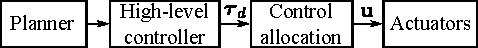
\includegraphics[width=.45\textwidth]{figures/ccta/diagram.pdf}
    \vspace{-1mm}
    \caption{Control system of overactuated vehicles considered in this chapter}
    \label{fig:ccta_diagram}
\end{figure}

The main contribution of this chapter is a reactive \acrfull{colav} algorithm that is included at the lowest level in the control pipeline, \emph{i.e.} in the control allocation, to ensure the safety of the vehicle regarding collision avoidance.
Since it is included at the lowest-possible control level, it also ensures the ``baseline'' safety of any other higher level (long term/deliberate) planners of the vehicle guidance, navigation and control system.
The algorithm can easily be implemented on vehicles that apply a numerical optimization-based method to control allocation.
Moreover, the algorithm does not rely on any communication between the vehicles; the only required information is the position and velocity of other vehicles.
The chapter extends the results in \cite{thyri_reactive_2020}, which only considers \acrfullpl{asv} and simple encounters between one \gls{asv} and a vessel moving at a constant course and speed, making the method applicable to a wider range of vehicles and scenarios with multiple autonomous vehicles.

The remainder of the chapter is organized as follows.
Section \ref{sec:ccta_model} defines the notation and describes the model of the vehicle.
The proposed control allocation method and \glspl{cbf} are introduced in Sections \ref{sec:ccta_alloc} and \ref{sec:ccta_CBF}.
%Section \ref{sec:ccta_alloc} introduces control allocation and Section \ref{sec:ccta_CBF} introduces CBFs.
Section \ref{sec:ccta_optimization} describes the resulting combined \gls{colav} and control allocation optimization problem.
Section \ref{sec:ccta_simulations} presents the results of numerical simulations using models of \glspl{asv}.
Finally, Section \ref{sec:ccta_conclusion} contains some concluding remarks.

\section{Vehicle Model}
\label{sec:ccta_model}

\subsection{Notation}
\label{sec:ccta_notation}

Let $\mathbf{p}$ denote the position and $\bs{\Theta}$ the orientation (expressed using the Euler angles) of the vehicle in a \acrfull{ned} reference frame.
%The test models presented in Section~\ref{sec:ccta_simulations} have three degrees of freedom (DOFs), with the position and orientation defined as follows
%\begin{align}
%    \mathbf{p} &= \left[ x ,\, y \right]^{\rm T}, &
%    \bs{\Theta} = \psi,
%\end{align}
%where $x$ is the North coordinate, $y$ is the East coordinate, and $\psi$ is the yaw angle.
%
Let $\pose$ be the pose of the vehicle
\begin{equation}
    \pose = \left[ \mathbf{p}^{\rm T} ,\, \bs{\Theta}^{\rm T} \right]^{\rm T}.
\end{equation}

Let $\vel$ be the velocities of the vehicle in the body-fixed frame.
%For our 3DOF models
%\begin{equation}
%    \vel = \left[ u ,\, v ,\, r \right]^{\rm T},
%\end{equation}
%where $u$ and $v$ are the surge and sway velocities, respectively, and $r$ is the yaw rate.
%
The complete state of the vehicle, $\mathbf{x}$, is defined as
\begin{equation}
    \mathbf{x} = \left[ \pose^{\rm T} \,, \vel^{\rm T} \right]^{\rm T}.
\end{equation}

Let $\bs{\tau}$ be the vector of generalized forces acting on the vehicle.
%For our 3DOF models
%\begin{equation}
%    \bs{\tau} = \left[ X ,\, Y ,\, N \right]^{\rm T},
%\end{equation}
%where $X$ and $Y$ are the forces in the surge and sway direction, respectively, and $N$ is the yaw moment.
Let $K$ be the number of actuator parameters and $\mathbf{u} \in \mathbb{R}^{K}$ the vector of inputs.
Furthermore, let $b : \mathbb{R}^{K} \rightarrow \mathbb{R}^{n_{\rm DOF}}$ be a nonlinear function that maps the inputs to the generalized forces ($n_{\rm DOF}$ is the number of \glspl{dof}).

\subsection{Equations of Motion}

The time-derivative of the pose can be obtained by transforming the velocities. % to the NED frame.
In addition, we assume that the time-derivatives of the velocities are affine in the generalized forces.
We thus consider vehicles described by the following dynamical equations
\begin{equation}
    \dot{\mathbf{x}} = \begin{bmatrix} \dot{\pose} \\ \dot{\vel} \end{bmatrix} = \begin{bmatrix}
        \mathbf{J}(\bs{\Theta})\,\vel \\ f(\mathbf{x}) + g(\mathbf{x})\,\bs{\tau}
    \end{bmatrix} = \begin{bmatrix}
        \mathbf{J}(\bs{\Theta})\,\vel \\ f(\mathbf{x}) + g(\mathbf{x})\,b(\mathbf{u})
    \end{bmatrix},
    \label{eq:ccta_affine_model}
\end{equation}

\noindent where $\mathbf{J}(\bs{\Theta})$ is the transformation matrix. % from body-fixed to NED frame. 
This equation describes a large class of systems, including the matrix-vector model of marine vessels \cite{fossen_handbook_2011}
\begin{subequations}
    \begin{align}
        \dot{\pose} &= \mathbf{J}(\bs{\Theta})\,\vel, \\
        \mathbf{M}\,\dot{\vel} + \left(\mathbf{C}(\vel) + \mathbf{D}(\vel)\right)\,\vel + \mathbf{g}(\pose) &= b(\mathbf{u}),% + \bs{\tau}_w,
    \end{align}
    \label{eq:ccta_matrix_model}
    \vspace{-4mm}
\end{subequations}

\noindent This model can be converted to the form in \eqref{eq:ccta_affine_model} since the matrix $\mathbf{M}$ is invertible.

\section{Control Allocation}
\label{sec:ccta_alloc}

As stated in the Introduction, the goal of the control allocation is to find the inputs that generate the desired forces given by the high-level controller.
For details on control allocation techniques for both linear and nonlinear systems, the reader is referred to \cite{johansen_control_2013}.

In this chapter, we consider systems where the function $b$ can be nonlinear.
In the literature, nonlinear control allocation is commonly solved by linearizing the function $b$ \cite{harkegard_dynamic_2004,johansen_constrained_2004}%, \emph{i.e.,}
\begin{equation}
    b(\mathbf{u}_0 + \Delta\mathbf{u}) \approx b(\mathbf{u}_0) + \mathbf{B}(\mathbf{u}_0)\,\Delta\mathbf{u},
    \label{eq:ccta_forces_approximation}
\end{equation}
where $\mathbf{u}_0$ are the inputs around which we linearize, $\Delta\mathbf{u}$ is the increment, and
\begin{equation}
    \mathbf{B}(\mathbf{u}_0) = \frac{\partial b(\mathbf{u})}{\partial \mathbf{u}}\bigg|_{\mathbf{u}_0},
\end{equation}
is the Jacobian of $b$ evaluated at $\mathbf{u}_0$.
Let $\bs{\tau}_d$ be the desired forces.
The goal of our control allocation scheme is to find optimal inputs $\mathbf{u}^*$ that satisfy
\begin{equation}
    \mathbf{u}^* = \argmin_{\mathbf{u}\in\mathbb{R}^{K}}\,\left\| b(\mathbf{u}) - \bs{\tau}_d \right\|^2.
\end{equation}

Using the approximation \eqref{eq:ccta_forces_approximation}, we can formulate the control allocation problem as a \acrfull{qp} 
\begin{align}
    \mathbf{u}^* &= \mathbf{u}_0 + \Delta\mathbf{u}^*, \\
    \Delta\mathbf{u}^* &= \argmin_{\Delta\mathbf{u}\in\mathbb{R}^{K}}\,\left\| b(\mathbf{u}_{0}) + \mathbf{B}(\mathbf{u}_{0})\,\Delta\mathbf{u} - \bs{\tau}_{d} \right\|^2.
\end{align} 

\section{Control Barrier Functions}
\label{sec:ccta_CBF}
In this section, we will briefly present the theory behind \acrfullpl{cbf}.
For more details, the reader is referred to \cite{ames_control_2019}.
After presenting the notation for multiple vehicles, we define the \gls{cbf} for \gls{colav}.

\subsection{Introduction to CBFs}
Consider a nonlinear control-affine system
\begin{equation}
    \dot{\mathbf{x}} = \widetilde{f}(\mathbf{x}) + \widetilde{g}(\mathbf{x})\,\mathbf{u},
    \label{eq:ccta_control_affine_system}
\end{equation}
\noindent where $\mathbf{x} \in \mathbb{R}^n$.
Suppose that the system must satisfy a safety constraint
$
    h(\mat{x}) \geq 0,
$
where $h : \mathbb{R}^{n} \rightarrow \mathbb{R}$ is the so-called \emph{barrier function}.
Then, we can define the so-called \emph{safe set}, a set of all states that satisfy the safety constraint, as
\begin{equation}
    \mathcal{C} = \left\{ \mathbf{x} \,|\, h(\mathbf{x}) \geq 0 \right\}.
\end{equation}
If the initial condition of the system \eqref{eq:ccta_control_affine_system} lies in the safe set, the system trajectory will stay within $\mathcal{C}$ if the following inequality holds \cite{ames_control_2019}
\begin{equation}
    \frac{{\rm d}}{{\rm d}t}h(\mathbf{x}) = \frac{\partial h(\mathbf{x})}{\partial \mathbf{x}}\,\left(\widetilde{f}(\mathbf{x}) + \widetilde{g}(\mathbf{x})\,\mathbf{u}\right) \geq - \gamma\bigl(h(\mathbf{x})\bigr),
    \label{eq:ccta_cbf_inequality}
\end{equation}
where $\gamma$ is an extended class-$\mathcal{K}_{\infty}$ function. 
If there exists an input $\mathbf{u}$ such that \eqref{eq:ccta_cbf_inequality} is satisfied, then $h$ is a valid \gls{cbf} for the system \eqref{eq:ccta_control_affine_system}.

\subsection{CBFs for Reactive Collision Avoidance}
%First, we need to extend the notation from Section~\ref{sec:ccta_notation} to multi-vehicle systems.
Let there be $N$ vehicles.
We shall denote the variables that belong to a given vehicle by a lower index (\emph{e.g.,} $\mathbf{x}_{i}$ is the state of the $i^{\rm th}$ vehicle).
In addition, let us define a relative position of vehicles $i$ and $j$ as
\begin{equation}
    \mathbf{p}_{ij} = \mathbf{p}_{i} - \mathbf{p}_{j}.
    \label{eq:ccta_p_ij}
\end{equation}

To ensure safety, we need a collection of \glspl{cbf} that enforce safe distances between each pair of vehicles.
In the literature, vehicles described by the model \eqref{eq:ccta_affine_model} frequently use \glspl{cbf} in the following form \cite{basso_safety-critical_2020,thyri_reactive_2020}
\begin{equation}
    %h_{ij}(\mathbf{x}_{i}, \mathbf{x}_{j}) = \|\mathbf{p}_{ij}\| - d_{\min} + k_v\,\frac{1}{\|\mathbf{p}_{ij}\|}\,\mathbf{p}_{ij}_{\rm T}\,\dot{\mathbf{p}}_{ij},
    h_{ij}(\mathbf{x}_{i}, \mathbf{x}_{j}) = \|\mathbf{p}_{ij}\| - d_{\min} + k_v\,\frac{\rm d}{{\rm d}t}\|\mathbf{p}_{ij}\|,
    \label{eq:ccta_CBF}
\end{equation}
where $d_{\min}$ is a minimum safe distance, and $k_v$ is a coefficient that penalizes the relative speed of the vehicles.

To use $h_{ij}$ as a control barrier function, we need to calculate its time-derivative.
Differentiating \eqref{eq:ccta_CBF} with respect to time yields
\begin{equation}
    \frac{\rm d}{{\rm d}t}h_{ij}(\mathbf{x}_{i}, \mathbf{x}_{j}) = \frac{\rm d}{{\rm d}t}\|\mathbf{p}_{ij}\| + k_v\,\frac{\rm d_2}{{\rm d}t_2}\|\mathbf{p}_{ij}\|.
\end{equation}

%Note that the norm $\|\mathbf{p}_{ij}\|$ can be defined as
%\begin{equation}
%    \|\mathbf{p}_{ij}\| = \sqrt{(\mathbf{p}_{ij})_{\rm T}\,\mathbf{p}_{ij}}.
%\end{equation}

%By applying the chain rule, we get
%\begin{align}
%    \frac{\rm d}{{\rm d}t}\|\mathbf{p}_{ij}\| &= \frac{1}{\|\mathbf{p}_{ij}\|}\,(\mathbf{p}_{ij})_{\rm T}\,\dot{\mathbf{p}}_{ij}, \\
%    \begin{split}
%        \frac{\rm d_2}{{\rm d}t_2}\|\mathbf{p}_{ij}\| &=  - \frac{1}{\|\mathbf{p}_{ij}\|_3}\,\left((\mathbf{p}_{ij})_{\rm T}\,\dot{\mathbf{p}}_{ij}\right)_2 \\
%        +&\frac{1}{\|\mathbf{p}_{ij}\|}\,\left((\dot{\mathbf{p}}_{ij})_{\rm T}\,\dot{\mathbf{p}}_{ij} + (\mathbf{p}_{ij})_{\rm T}\,\ddot{\mathbf{p}}_{ij}\right).
%    \end{split}        
%\end{align}

To calculate the first and second time-derivative of the relative distance, we need to find the first and second time-derivatives of the relative position.
For $\dot{\mathbf{p}}_{ij}$, we split the derivative of $\pose$ from \eqref{eq:ccta_affine_model} into the derivatives of position and orientation \vspace{-2mm}
\begin{equation}
    \dot{\pose}_{i} = \begin{bmatrix} \dot{\mathbf{p}}_{i} \\ \dot{\bs{\Theta}}_{i} \end{bmatrix} = \begin{bmatrix}
        \mathbf{J}_{\mathbf{p}}(\bs{\Theta}_{i}) \\ \mathbf{J}_{\bs{\Theta}}(\bs{\Theta}_{i})
    \end{bmatrix}\,\vel_{i}.
\end{equation}

\noindent Substituting this into the time-derivative of \eqref{eq:ccta_p_ij} yields
\begin{equation}
    \dot{\mathbf{p}}_{ij} = \mathbf{J}_{\mathbf{p}}(\bs{\Theta}_{i}) \, \vel_{i} - \mathbf{J}_{\mathbf{p}}(\bs{\Theta}_{j}) \, \vel_{j}.
    \label{eq:ccta_p_dot}
\end{equation}

\noindent For $\ddot{\mathbf{p}}_{ij}$, we assume that the target maintains its velocity, \emph{i.e.,}
\begin{equation}
    \ddot{\mathbf{p}}_{ij} \approx \ddot{\mathbf{p}}_{i},
\end{equation}
when calculating the time-derivative for the $i^{\rm th}$ vehicle.
As discussed in \cite{thyri_reactive_2020}, this is a ``mild worst-case'' assumption, since maneuvers of the target vehicle tend to aid to resolving the situation.
Thus, taking the time-derivative of \eqref{eq:ccta_p_dot} yields
\begin{equation}
    \ddot{\mathbf{p}}_{i} = \dot{\mathbf{J}}_{\mathbf{p}}(\bs{\Theta}_{i}) \, \vel_{i} + \mathbf{J}_{\mathbf{p}}(\bs{\Theta}_{i}) \, \dot{\vel}_{i}.
    \label{eq:ccta_p_ddot}
\end{equation}

Finally, we substitute the approximation of forces from \eqref{eq:ccta_forces_approximation} into the equation for $\dot{\vel}$ in \eqref{eq:ccta_affine_model} to get
\begin{equation}
    \dot{\vel}_{i} = f(\mathbf{x}_{i}) + g(\mathbf{x}_{i})\,\left(b(\mathbf{u}_{0,i}) + \mathbf{B}(\mathbf{u}_{0,i})\,\Delta\mathbf{u}_{i}\right),
\end{equation}
which we can substitute into \eqref{eq:ccta_p_ddot} to calculate $\ddot{\mathbf{p}}_{i}$.

\section{Formulating the Optimization Problem}
\label{sec:ccta_optimization}
Now we can combine the definitions from Sections~\ref{sec:ccta_alloc} and \ref{sec:ccta_CBF} to formulate the proposed optimization problem for control allocation with multi-vehicle \gls{colav}.

\subsection{The Basic Optimization Problem}
Let $\mathbf{u}_{0,i}$ be the inputs of vehicle $i$ from the previous control period.
The new inputs are calculated as
\begin{equation}
    \mathbf{u}_{i} = \mathbf{u}_{0,i} + \Delta\mathbf{u}_{i}^*,
\end{equation}
where $\Delta\mathbf{u}_{i}^*$ is obtained by solving the following \gls{qp}
\begin{subequations}
    \begin{align}
        \Delta\mathbf{u}_{i}^* &= \argmin_{\Delta\mathbf{u}_{i}\in\mathbb{R}^{K}}\,\left\| b(\mathbf{u}_{0,i}) + \mathbf{B}(\mathbf{u}_{0,i})\,\Delta\mathbf{u}_{i} - \bs{\tau}_{d,i} \right\|^2\,, \label{eq:ccta_combined_avoidance_allocation_criterion} \\
        \begin{split}
            \text{s.t. }& \frac{{\rm d}}{{\rm d}t}h_{ij}(\mathbf{x}_{i}, \mathbf{x}_{j}) \geq - \gamma\left(h_{ij}(\mathbf{x}_{i}, \mathbf{x}_{j})\right), \\
            & j \in \left\{ 1, \ldots, N \right\} \setminus \left\{ i \right\},
        \end{split} \label{eq:ccta_combined_avoidance_allocation_constraint} \\
        & \mathbf{u}_{i,\min} \leq \mathbf{u}_{0,i} + \Delta\mathbf{u}_{i} \leq \mathbf{u}_{i,\max}, \\
        & \Delta\mathbf{u}_{i,\min} \leq \Delta\mathbf{u}_{i} \leq \Delta\mathbf{u}_{i,\max}, \label{eq:ccta_combined_avoidance_allocation_delta_u}
    \end{align}
    \label{eq:ccta_combined_avoidance_allocation}
\end{subequations}
\noindent where $\mathbf{u}_{i,\min}$ and $\mathbf{u}_{i,\max}$ are the absolute actuator limits, and $\Delta\mathbf{u}_{i,\min}$ and $\Delta\mathbf{u}_{i,\max}$ are the actuator rate limits.
The absolute limits are usually given by the physical limitations of the vehicle (\emph{e.g.,} the thrust of a propeller or the deflection of control surfaces) whereas the rate limits are user-defined to reduce the rapid changes that wear out the actuators.

Simulation results using this control allocation algorithm are presented in Section~\ref{sec:ccta_simulations}.

\subsection{Modified Optimization Problem}
The algorithm in \eqref{eq:ccta_combined_avoidance_allocation} is suitable for vehicles where the number of actuators is equivalent to the number of DOFs.
Applying the algorithm to vehicles where the number of actuators is much greater than the number of DOFs results in inefficient usage of the available actuators, as can be seen in Section~\ref{sec:ccta_simulations}.

To reduce this effect, we add penalty terms on the actuator usage, similar to those proposed in \cite{johansen_constrained_2004}, in the cost function.
To simplify the notation, let $\|\mathbf{x}\|_{\mathbf{Q}}^2$ be the squared norm of a vector $\mathbf{x}$ weighted by a matrix $\mathbf{Q}$, \emph{i.e.,}
\begin{equation}
    \|\mathbf{x}\|_{\mathbf{Q}}^2 = \mathbf{x}^{\rm T}\,\mathbf{Q}\,\mathbf{x}.
\end{equation}

The modified optimization problem is defined as follows
\begin{subequations}
    \begin{align}
    \begin{split}
        \Delta\mathbf{u}_{i}^* &= \argmin_{\Delta\mathbf{u}_{i}\in\mathbb{R}^{K}}\,\left\| b(\mathbf{u}_{i,0}) + \mathbf{B}(\mathbf{u}_{i,0})\,\Delta\mathbf{u}_{i} - \bs{\tau}_{d,i} \right\|_{\mathbf{Q}}^2 \\
        &\quad \quad \quad + \left\| \mathbf{u}_{0,i} + \Delta\mathbf{u}_{i} \right\|_{\mathbf{R}_{\rm abs}}^2 + \left\|\Delta\mathbf{u}_{i}\right\|_{\mathbf{R}_{\rm rel}}^2,
    \end{split} \\    
%    \begin{split}
%        \text{s.t. }& \frac{{\rm d}}{{\rm d}t}h^{ij}(\mathbf{x}^{i}, \mathbf{x}^{j}) \geq - \gamma\left(h^{ij}(\mathbf{x}^{i}, \mathbf{x}^{j})\right), \\
%        & j \in \left\{ 1, \ldots, n \right\} \setminus \left\{ i \right\},
%    \end{split} \\
%    & \mathbf{u}^{i}_{\min} \leq \mathbf{u}^{i}_{0} + \Delta\mathbf{u}^{i} \leq \mathbf{u}^{i}_{\max}, \\
%    & \Delta\mathbf{u}^{i}_{\min} \leq \Delta\mathbf{u}^{i} \leq \Delta\mathbf{u}^{i}_{\max},
    \text{s.t. }&\text{constraints \eqref{eq:ccta_combined_avoidance_allocation_constraint}--\eqref{eq:ccta_combined_avoidance_allocation_delta_u},}
    \end{align}
    \label{eq:ccta_combined_avoidance_allocation_modified}
\end{subequations}
\noindent where $\mathbf{Q}$ is a positive definite matrix that penalizes the difference between the desired and actual forces, and $\mathbf{R}_{\rm abs}$ and $\mathbf{R}_{\rm rel}$ are positive semidefinite matrices that penalize the absolute and incremental usage of actuators, respectively.

Note that both \eqref{eq:ccta_combined_avoidance_allocation} and \eqref{eq:ccta_combined_avoidance_allocation_modified} use only local information and measurements, and can thus be solved locally for each vehicle.

When choosing the weight matrices, we first note that the vector $\bs{\tau}$ contains both forces and torques.
The matrix $\mathbf{Q}$ should penalize them differently.
In the simulations in Section~\ref{sec:ccta_simulations}, we choose
\begin{equation}
   \mathbf{Q} = \diag{(1,1,\frac{1}{L^2})},
\end{equation}
where $\diag(.)$ is a diagonal matrix and $L$ is the smallest distance of the thrusters from the center of mass.

\section{Simulations}
\label{sec:ccta_simulations}
In the simulations, we test the ability of the proposed algorithms to resolve a situation when four surface vessels are simultaneously in danger of collision.
Each vessel starts in the corner of a square and is guided towards a reference located in the diagonally opposite corner.

We tested the proposed algorithms on two models of ASVs --- the \emph{milliAmpere} ferry \cite{pedersen_optimization_2019} and the $1:90$ scaled model of the Inocean Cat I drillship \cite{bjorno_thruster-assisted_2016} --- using Simulink.
Both vessels are equipped with azimuth thrusters; the \emph{milliAmpere} has two and the drillship has six.
Each thruster is parametrized by two values: its thrust force and its azimuth.
The input vector for these vessels is defined as \vspace{-2mm}
\begin{equation}
    \mathbf{u} = \left[ f_1 ,\, \ldots ,\, f_k ,\, \alpha_1 ,\, \ldots ,\, \alpha_k \right]^{\rm T},
\end{equation}
where $f_i$ is the thrust force and $\alpha_i$ is the azimuth angle of the $i^{\rm th}$ thruster, and $k$ is the number of thrusters.
%
Both ASV models have 3DOFs, \emph{i.e.,} the North-East position and the yaw angle.
The function that maps the inputs to the generalized forces is \vspace{-2mm}
\begin{equation}
    \scale[0.93]{b(\mathbf{u}) = \sum_{i=1}^k f_i \left[ \cos\alpha_i, \sin\alpha_i, L_x^i\,\sin\alpha_i - L_y^i\,\cos\alpha_i \right]^{\rm T},}
\end{equation}
where $L_x^i$ and $L_y^i$ is the position of the $i^{\rm th}$ thruster, relative to the center of mass.

For the higher-level controller that provides the desired forces, we use a nonlinear PID controller \cite{fossen_handbook_2011}.
The nonlinear PID is an output-linearizing controller that transforms the nonlinear dynamical equations from \eqref{eq:ccta_matrix_model} to
\begin{equation}
    \ddot{\pose} + 2\,\bs{\Omega}_n\,\mathbf{Z}\,\dot{\pose} + \bs{\Omega}_n^2\,\pose = 0,
\end{equation}
where $\mathbf{Z}$ is the diagonal relative damping matrix, and $\bs{\Omega}_n$ is the diagonal natural frequency matrix.
Both matrices are tuning parameters.
For convenience, we express $\bs{\Omega}_n$ in terms of a bandwidth matrix $\bs{\Omega}_{bw}$
\begin{equation}
    \bs{\Omega}_n = \bs{\Omega}_{bw} \, \left(\sqrt{\mathbf{I} - 2\,\mathbf{Z}^2 + \sqrt{4\,\mathbf{Z}^4 - 4\,\mathbf{Z}^2 + 2\,\mathbf{I}}}\right)^{-1},
\end{equation}
where $\sqrt{.}$ is an elementwise square root.

The simulation parameters for both vessels are summarized in Table~\ref{tab:params}.
% The matrix $\mathbf{Q}$ is chosen as
% \begin{align}
%     \mathbf{Q} &= \diag{\left( 1,1,\frac{1}{L^2} \right)},&
%     L &= \min_{i} \sqrt{\left(L_x^i\right)^2 + \left(L_y^i\right)^2}.
% \end{align}

\noindent Since the power consumption of a thruster increases with the absolute value of its thrust force and the increment of its azimuth, the matrices $\mathbf{R}_{\rm abs}$ and $\mathbf{R}_{\rm rel}$ are chosen as
%\begin{align}
%    \mathbf{R}_{\rm abs} &= \begin{bmatrix} r_{\rm abs}\,\mathbf{I}_{k} & \\ & \mathbf{0}_{k \times k} \end{bmatrix},
%    \mathbf{R}_{\rm rel} &= \begin{bmatrix} \mathbf{0}_{k \times k} & \\ & r_{\rm rel}\,\mathbf{I}_{k} \end{bmatrix},
%\end{align}
\begin{equation}
    \scale[0.931]{\mathbf{R}_{\rm abs} = \begin{bmatrix} r_{\rm abs}\,\mathbf{I}_{k} & \mathbf{O}_{k \times k} \\ \mathbf{O}_{k \times k} & \mathbf{O}_{k \times k} \end{bmatrix}, \,
    \mathbf{R}_{\rm rel} = \begin{bmatrix} \mathbf{O}_{k \times k} & \mathbf{O}_{k \times k} \\ \mathbf{O}_{k \times k} & r_{\rm rel}\,\mathbf{I}_{k} \end{bmatrix},}
\end{equation}
The rate constraints are identical for all thrusters and symmetric, \emph{i.e.,}
\begin{align}
    \Delta\mathbf{u}_{\max} &= \begin{bmatrix} \Delta f_{\max}\,\mathbf{1}_k \\ \Delta \alpha_{\max}\,\mathbf{1}_k \end{bmatrix}, &
    \Delta\mathbf{u}_{\min} &= - \Delta\mathbf{u}_{\max},
\end{align}
where $\Delta f_{\max}$ and $\Delta \alpha_{\max}$ are the force and azimuth rate constraints, respectively, and $\mathbf{1}_k$ is a vector of ones.

\begin{table}[t]
    \centering
    \begin{tabular}{cc|rrr}
        \multirow{2}{*}{\textbf{Vessel}} & \multirow{2}{*}{\textbf{Scenario}} & \multicolumn{3}{|c}{\textbf{Thruster utilization [\%]}} \\
        & & \textbf{Maximum} & \textbf{Minimum} & \textbf{Mean} \\ \hline
        \multirow{2}{*}{\textbf{milliAmpere}} & \textbf{basic} & $2.074$ & $1.550$ & $1.822$ \\
        & \textbf{modified} & $0.838$ & $0.835$ & $0.837$ \\
        \multirow{2}{*}{\textbf{drillship}} & \textbf{basic} & $100.000$ & $1.282$ & $51.496$ \\
        & \textbf{modified} & $6.161$ & $0.259$ & $3.816$ 
    \end{tabular}
    \caption{Steady-state thruster utilization of the \emph{basic} algorithm \eqref{eq:ccta_combined_avoidance_allocation} and the \emph{modified} algorithm \eqref{eq:ccta_combined_avoidance_allocation_modified}.}
    \label{tab:thruster_utilization}
    \vspace{-5mm}
\end{table}

\begin{table}[b]
    \centering
    \begin{tabular}{c|cc}
        {\bf Parameter} & {\bf \emph{milliAmpere}} & {\bf drillship} \\ \hline
        %$\bs{\Omega}_{bw}$ & $\diag{(0.1,\,0.1,\,0.5)}$ & $\diag{(0.1,\,0.1,\,0.5)}$ \\
        $\bs{\Omega}_{bw}$ & \multicolumn{2}{c}{$\diag{(0.1,\,0.1,\,0.5)}$} \\
        %$\mathbf{Z}$ & $\diag{(0.95,\,0.95,\,0.97)}$ & $\diag{(0.95,\,0.95,\,0.97)}$ \\
        $\mathbf{Z}$ & \multicolumn{2}{c}{$\diag{(0.95,\,0.95,\,0.97)}$} \\
        $\mathbf{Q}$ & $\diag{(1,1,0.7)}$ & $\diag{(1,1,1.13)}$ \\
        %$\mathbf{R}_{\rm abs}$ & $\begin{bmatrix} \mathbf{I}_{2 \times 2} & \\ & \mathbf{0}_{2 \times 2} \end{bmatrix}$ & $\begin{bmatrix} \mathbf{I}_{6 \times 6} & \\ & \mathbf{0}_{6 \times 6} \end{bmatrix}$ \\
        $r_{\rm abs}$ & $1$ & $1$ \\
        %$\mathbf{R}_{\rm rel}$ & $\begin{bmatrix} \mathbf{0}_{2 \times 2} & \\ & 100\mathbf{I}_{2 \times 2} \end{bmatrix}$ & $\begin{bmatrix} \mathbf{0}_{6 \times 6} & \\ & \mathbf{I}_{6 \times 6} \end{bmatrix}$ \\
        $r_{\rm rel}$ & $100$ & $1$ \\
        $d_{\min} \, [{\rm m}]$ & $15$ & $2.5$ \\
        $k_v \, [{\rm s}]$ & $15$ & $15$ \\
        $\gamma(h)$ & $0.1\,h$ & $0.1\,h$ \\
        $f_{\min} \, [{\rm N}]$ & $-350$ & $-0.8$ \\
        $f_{\max} \, [{\rm N}]$ & $500$ & $1.5$ \\
        $\Delta f_{\max} \, [{\rm N}]$ & $350$ & $0.5$ \\
        $\Delta \alpha_{\max} \, [{\rm rad}]$ & $\frac{\pi}{8}$ & $\frac{\pi}{8}$
    \end{tabular}
    \caption{Simulation parameters. Parameters $\bs{\Omega}_{bw}$ and $\bs{Z}$ are identical for both scenarios, $\diag{(.)}$ is a diagonal matrix}
    \label{tab:params}
\end{table}

The results of the simulations are shown in Figures \ref{fig:ccta_orig}, \ref{fig:ccta_modified}, and \ref{fig:ccta_uncontrolled}.
Figure \ref{fig:ccta_orig} shows the results of algorithm \eqref{eq:ccta_combined_avoidance_allocation}.
Figure \ref{fig:ccta_modified} shows the results of algorithm \eqref{eq:ccta_combined_avoidance_allocation_modified}.
Each figure consists of two plots.
The plot on the left displays the trajectory of the vessels.
The colored lines show the trajectory of each vessel, the boat-shaped polygons represent the pose of the vessels at several evenly spaced time-instances, and the colored crosses show the reference of each vessel.
The plot on the right shows the smallest distance between the vessels compared to the minimum safe distance $d_{\min}$.
In both scenarios, the vessels reach their reference position while maintaining safe distance.

We also tested a scenario where one of the vessels is uncontrolled.
The results are shown in Figure~\ref{fig:ccta_uncontrolled}.
In this scenario, the uncontrolled vessel (plotted in black) solves the control allocation problem without the \gls{cbf} constraints \eqref{eq:ccta_combined_avoidance_allocation_constraint}.
Although the time it takes the vessels to converge to their goal positions is greater, the minimum safe distance is still maintained.

In this section, we have provided some insight into how to chose some of the parameters for the simulated models.
When it comes to the choice of the coefficient $k_v$, introduced in \eqref{eq:ccta_CBF}, and the extended class-$\mathcal{K}_{\infty}$ function $\gamma$, introduced in \eqref{eq:ccta_combined_avoidance_allocation}, the following considerations can be made.
Intuitively, increasing $k_v$ increases the size of the ``unsafe'' region where the barrier function is negative, causing the system to react sooner in situations where two vehicles are on collision course.
Conversely, increasing the slope of $\gamma$ decreases the size of the region where the constraint \eqref{eq:ccta_combined_avoidance_allocation_constraint} is active, causing the system to react later.

\pgfplotsset{table/search path={figures/ccta/data}}
\begin{figure*}[t]
    \centering
    \begin{subfigure}{\linewidth}
        \centering
        %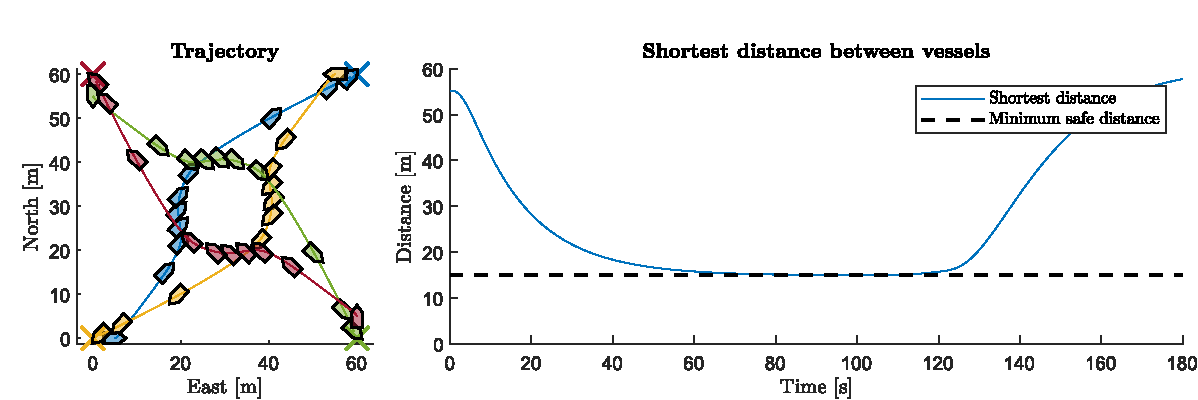
\includegraphics[width = \textwidth]{figures/ccta/milliAmpere_orig.pdf}
        % This file was created by matlab2tikz.
%
%The latest updates can be retrieved from
%  http://www.mathworks.com/matlabcentral/fileexchange/22022-matlab2tikz-matlab2tikz
%where you can also make suggestions and rate matlab2tikz.
%
\definecolor{mycolor1}{rgb}{0.00000,0.44700,0.74100}%
\definecolor{mycolor2}{rgb}{0.85000,0.32500,0.09800}%
\definecolor{mycolor3}{rgb}{0.92900,0.69400,0.12500}%
\definecolor{mycolor4}{rgb}{0.49400,0.18400,0.55600}%

%
\begin{tikzpicture}

\begin{axis}[%
width=0.24\textwidth,
height=0.24\textwidth,
at={(0,0)},
scale only axis,
xmin=-2,
xmax=62,
xlabel style={font=\color{white!15!black}\small, yshift=1.5mm},
xlabel={East [m]},
ticklabel style={font=\small},
ymin=-2,
ymax=62,
ylabel style={font=\color{white!15!black}\small, yshift=-1.5mm},
ylabel={North [m]},
axis background/.style={fill=white},
title style={font=\bfseries, yshift=-2.5mm},
title={Trajectory},
xmajorgrids,
ymajorgrids,
]
\def\nboatplots{7}

\addplot [color=mycolor1, line width=0.8pt]
  table[]{milliAmpere_orig-1.tsv};
\foreach \i in {1,...,\nboatplots}
  \addplot[area legend, draw=black, fill=mycolor1, fill opacity=0.75, line width=0.5pt]
  table[x=x\i, y=y\i]{milliAmpere_orig-asv-1.tsv};

\addplot [color=mycolor2, line width=0.8pt]
  table[]{milliAmpere_orig-2.tsv};
\foreach \i in {1,...,\nboatplots}
  \addplot[area legend, draw=black, fill=mycolor2, fill opacity=0.75, line width=0.5pt]
  table[x=x\i, y=y\i]{milliAmpere_orig-asv-2.tsv};

\addplot [color=mycolor3, line width=0.8pt]
  table[]{milliAmpere_orig-3.tsv};
\foreach \i in {1,...,\nboatplots}
  \addplot[area legend, draw=black, fill=mycolor3, fill opacity=0.75, line width=0.5pt]
  table[x=x\i, y=y\i]{milliAmpere_orig-asv-3.tsv};

\addplot [color=mycolor4, line width=0.8pt]
  table[]{milliAmpere_orig-4.tsv};
\foreach \i in {1,...,\nboatplots}
  \addplot[area legend, draw=black, fill=mycolor4, fill opacity=0.75, line width=0.5pt]
  table[x=x\i, y=y\i]{milliAmpere_orig-asv-4.tsv};

\end{axis}

\begin{axis}[%
width=0.55\textwidth,
height=0.24\textwidth,
at={(0.35\textwidth,0)},
scale only axis,
xmin=0,
xmax=180,
xlabel style={font=\color{white!15!black}\small, yshift=1.5mm},
xlabel={Time [s]},
ymin=0,
ymax=60,
xmajorgrids,
ymajorgrids,
ticklabel style={font=\small},
ylabel style={font=\color{white!15!black}\small, yshift=-1.5mm},
ylabel={Distance [m]},
axis background/.style={fill=white},
title style={font=\bfseries, yshift=-2mm},
title={Shortest distance between vessels},
legend style={/tikz/column 2/.style={column sep=5pt,}, font=\small, at={(0.75,0.95)}, anchor=north east},
]
\addplot [color=mycolor1, line width=0.8pt]
  table[]{milliAmpere_orig-5.tsv};
\addlegendentry{Shortest distance}

\addplot [color=black, dashed, line width=1.5pt]
  table[]{milliAmpere_orig-6.tsv};
\addlegendentry{Minimum distance}

\end{axis}
\end{tikzpicture}%
        \vspace{-0.5em}
        \caption{Algorithm \eqref{eq:ccta_combined_avoidance_allocation} on four \emph{milliAmpere} vessels}
        %\vspace*{1em}
    \end{subfigure}
    \vspace{-1em}
    \begin{subfigure}{\linewidth}
        \centering
        %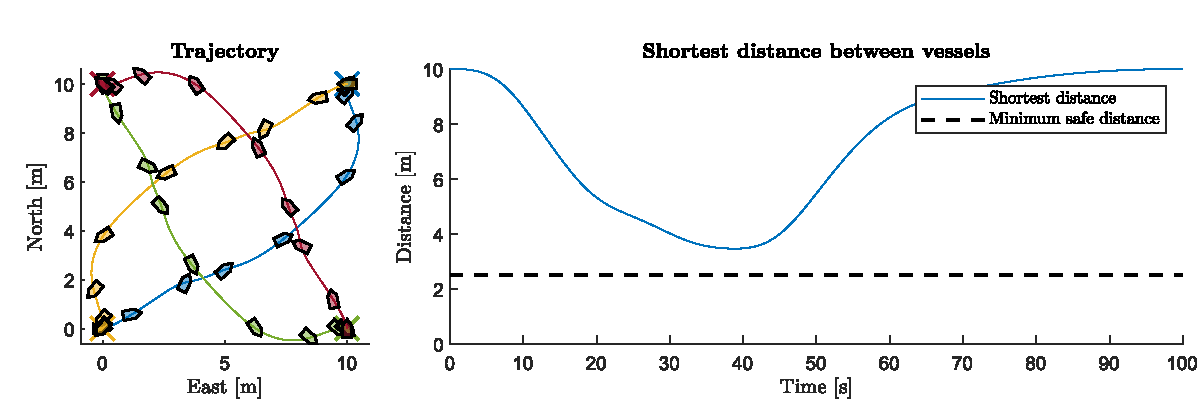
\includegraphics[width = \textwidth]{figures/ccta/drillship_orig.pdf}
        % This file was created by matlab2tikz.
%
%The latest updates can be retrieved from
%  http://www.mathworks.com/matlabcentral/fileexchange/22022-matlab2tikz-matlab2tikz
%where you can also make suggestions and rate matlab2tikz.
%
\definecolor{mycolor1}{rgb}{0.00000,0.44700,0.74100}%
\definecolor{mycolor2}{rgb}{0.85000,0.32500,0.09800}%
\definecolor{mycolor3}{rgb}{0.92900,0.69400,0.12500}%
\definecolor{mycolor4}{rgb}{0.49400,0.18400,0.55600}%

%
\begin{tikzpicture}

\begin{axis}[%
width=0.24\textwidth,
height=0.24\textwidth,
at={(0,0)},
scale only axis,
xmin=-1,
xmax=11,
xlabel style={font=\color{white!15!black}\small, yshift=1.5mm},
xlabel={East [m]},
ticklabel style={font=\small},
ymin=-1,
ymax=11,
ylabel style={font=\color{white!15!black}\small, yshift=-3mm},
ylabel={North [m]},
axis background/.style={fill=white},
title style={font=\bfseries, yshift=-2.5mm},
title={Trajectory},
xmajorgrids,
ymajorgrids,
]
\def\nboatplots{10}

\addplot [color=mycolor1, line width=0.8pt]
  table[]{drillship_orig-1.tsv};
\foreach \i in {1,...,\nboatplots}
  \addplot[area legend, draw=black, fill=mycolor1, fill opacity=0.75, line width=0.5pt]
  table[x=x\i, y=y\i]{drillship_orig-asv-1.tsv};

\addplot [color=mycolor2, line width=0.8pt]
  table[]{drillship_orig-2.tsv};
\foreach \i in {1,...,\nboatplots}
  \addplot[area legend, draw=black, fill=mycolor2, fill opacity=0.75, line width=0.5pt]
  table[x=x\i, y=y\i]{drillship_orig-asv-2.tsv};

\addplot [color=mycolor3, line width=0.8pt]
  table[]{drillship_orig-3.tsv};
\foreach \i in {1,...,\nboatplots}
  \addplot[area legend, draw=black, fill=mycolor3, fill opacity=0.75, line width=0.5pt]
  table[x=x\i, y=y\i]{drillship_orig-asv-3.tsv};

\addplot [color=mycolor4, line width=0.8pt]
  table[]{drillship_orig-4.tsv};
\foreach \i in {1,...,\nboatplots}
  \addplot[area legend, draw=black, fill=mycolor4, fill opacity=0.75, line width=0.5pt]
  table[x=x\i, y=y\i]{drillship_orig-asv-4.tsv};

\end{axis}

\begin{axis}[%
width=0.55\textwidth,
height=0.24\textwidth,
at={(0.35\textwidth,0)},
scale only axis,
xmin=0,
xmax=100,
xlabel style={font=\color{white!15!black}\small, yshift=1.5mm},
xlabel={Time [s]},
ymin=0,
ymax=10,
xmajorgrids,
ymajorgrids,
ticklabel style={font=\small},
ylabel style={font=\color{white!15!black}\small, yshift=-1.75mm},
ylabel={Distance [m]},
axis background/.style={fill=white},
title style={font=\bfseries, yshift=-2mm},
title={Shortest distance between vessels},
legend style={/tikz/column 2/.style={column sep=5pt,}, font=\small, at={(0.99,0.65)}, anchor=north east},
]
\addplot [color=mycolor1, line width=0.8pt]
  table[]{drillship_orig-5.tsv};
%\addlegendentry{Shortest distance}

\addplot [color=black, dashed, line width=1.5pt]
  table[]{drillship_orig-6.tsv};
%\addlegendentry{Minimum distance}

\end{axis}
\end{tikzpicture}%
        \vspace{-2em}
        \caption{Algorithm \eqref{eq:ccta_combined_avoidance_allocation} on four drillships}
    \end{subfigure}
    \caption{Simulations of the control allocation algorithm \eqref{eq:ccta_combined_avoidance_allocation}}
    \label{fig:ccta_orig}
\end{figure*}

\begin{figure*}[t]
    \centering
    \begin{subfigure}{\linewidth}
        \centering
        %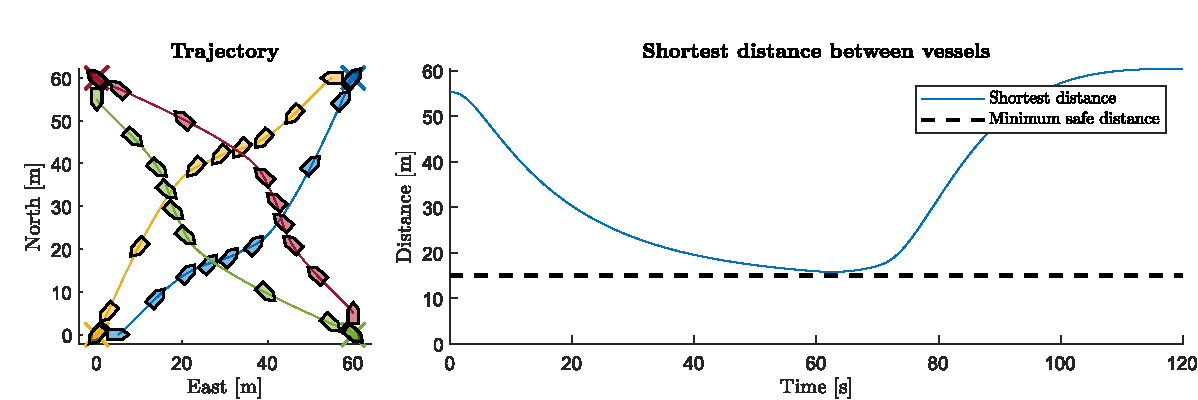
\includegraphics[width = \textwidth]{figures/ccta/milliAmpere_modified.pdf}
        % This file was created by matlab2tikz.
%
%The latest updates can be retrieved from
%  http://www.mathworks.com/matlabcentral/fileexchange/22022-matlab2tikz-matlab2tikz
%where you can also make suggestions and rate matlab2tikz.
%
\definecolor{mycolor1}{rgb}{0.00000,0.44700,0.74100}%
\definecolor{mycolor2}{rgb}{0.85000,0.32500,0.09800}%
\definecolor{mycolor3}{rgb}{0.92900,0.69400,0.12500}%
\definecolor{mycolor4}{rgb}{0.49400,0.18400,0.55600}%

%
\begin{tikzpicture}

\begin{axis}[%
width=0.24\textwidth,
height=0.24\textwidth,
at={(0,0)},
scale only axis,
xmin=-2,
xmax=62,
xlabel style={font=\color{white!15!black}\small, yshift=1.5mm},
xlabel={East [m]},
ticklabel style={font=\small},
ymin=-2,
ymax=62,
ylabel style={font=\color{white!15!black}\small, yshift=-1.5mm},
ylabel={North [m]},
axis background/.style={fill=white},
title style={font=\bfseries, yshift=-2.5mm},
title={Trajectory},
xmajorgrids,
ymajorgrids,
]
\def\nboatplots{10}

\addplot [color=mycolor1, line width=0.8pt]
  table[]{milliAmpere_modified-1.tsv};
\foreach \i in {1,...,\nboatplots}
  \addplot[area legend, draw=black, fill=mycolor1, fill opacity=0.75, line width=0.5pt]
  table[x=x\i, y=y\i]{milliAmpere_modified-asv-1.tsv};

\addplot [color=mycolor2, line width=0.8pt]
  table[]{milliAmpere_modified-2.tsv};
\foreach \i in {1,...,\nboatplots}
  \addplot[area legend, draw=black, fill=mycolor2, fill opacity=0.75, line width=0.5pt]
  table[x=x\i, y=y\i]{milliAmpere_modified-asv-2.tsv};

\addplot [color=mycolor3, line width=0.8pt]
  table[]{milliAmpere_modified-3.tsv};
\foreach \i in {1,...,\nboatplots}
  \addplot[area legend, draw=black, fill=mycolor3, fill opacity=0.75, line width=0.5pt]
  table[x=x\i, y=y\i]{milliAmpere_modified-asv-3.tsv};

\addplot [color=mycolor4, line width=0.8pt]
  table[]{milliAmpere_modified-4.tsv};
\foreach \i in {1,...,\nboatplots}
  \addplot[area legend, draw=black, fill=mycolor4, fill opacity=0.75, line width=0.5pt]
  table[x=x\i, y=y\i]{milliAmpere_modified-asv-4.tsv};

\end{axis}

\begin{axis}[%
width=0.535\textwidth,
height=0.24\textwidth,
at={(0.35\textwidth,0)},
scale only axis,
xmin=0,
xmax=120,
xlabel style={font=\color{white!15!black}\small, yshift=1.5mm},
xlabel={$t$ [s]},
ymin=0,
ymax=60,
xmajorgrids,
ymajorgrids,
ticklabel style={font=\small},
ylabel style={font=\color{white!15!black}\small, yshift=-1.5mm},
ylabel={Distance [m]},
axis background/.style={fill=white},
title style={font=\bfseries, yshift=-2mm},
title={Shortest distance between vessels},
legend style={/tikz/column 2/.style={column sep=5pt,}, font=\small, at={(0.68,0.95)}, anchor=north east},
]
\addplot [color=mycolor1, line width=0.8pt]
  table[]{milliAmpere_modified-5.tsv};
\addlegendentry{Shortest distance}

\addplot [color=black, dashed, line width=1.5pt]
  table[]{milliAmpere_modified-6.tsv};
\addlegendentry{Minimum distance}

\end{axis}
\end{tikzpicture}%
        \caption{Algorithm \eqref{eq:ccta_combined_avoidance_allocation_modified} on four \emph{milliAmpere} vessels}
        \vspace*{1em}
    \end{subfigure}
    \begin{subfigure}{\linewidth}
        \centering
        %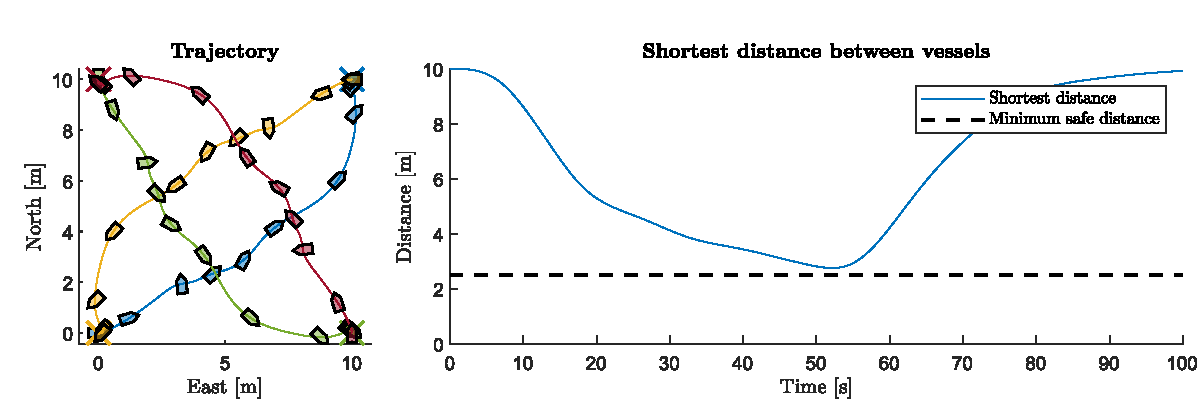
\includegraphics[width = \textwidth]{figures/ccta/drillship_modified.pdf}
        % This file was created by matlab2tikz.
%
%The latest updates can be retrieved from
%  http://www.mathworks.com/matlabcentral/fileexchange/22022-matlab2tikz-matlab2tikz
%where you can also make suggestions and rate matlab2tikz.
%
\definecolor{mycolor1}{rgb}{0.00000,0.44700,0.74100}%
\definecolor{mycolor2}{rgb}{0.85000,0.32500,0.09800}%
\definecolor{mycolor3}{rgb}{0.92900,0.69400,0.12500}%
\definecolor{mycolor4}{rgb}{0.49400,0.18400,0.55600}%

%
\begin{tikzpicture}

\begin{axis}[%
width=0.24\textwidth,
height=0.24\textwidth,
at={(0,0)},
scale only axis,
xmin=-1,
xmax=11,
xlabel style={font=\color{white!15!black}\small, yshift=1.5mm},
xlabel={East [m]},
ticklabel style={font=\small},
ymin=-1,
ymax=11,
ylabel style={font=\color{white!15!black}\small, yshift=-3mm},
ylabel={North [m]},
axis background/.style={fill=white},
title style={font=\bfseries, yshift=-2.5mm},
title={Trajectory},
xmajorgrids,
ymajorgrids,
]
\def\nboatplots{10}

\addplot [color=mycolor1, line width=0.8pt]
  table[]{drillship_modified-1.tsv};
\foreach \i in {1,...,\nboatplots}
  \addplot[area legend, draw=black, fill=mycolor1, fill opacity=0.75, line width=0.5pt]
  table[x=x\i, y=y\i]{drillship_modified-asv-1.tsv};

\addplot [color=mycolor2, line width=0.8pt]
  table[]{drillship_modified-2.tsv};
\foreach \i in {1,...,\nboatplots}
  \addplot[area legend, draw=black, fill=mycolor2, fill opacity=0.75, line width=0.5pt]
  table[x=x\i, y=y\i]{drillship_modified-asv-2.tsv};

\addplot [color=mycolor3, line width=0.8pt]
  table[]{drillship_modified-3.tsv};
\foreach \i in {1,...,\nboatplots}
  \addplot[area legend, draw=black, fill=mycolor3, fill opacity=0.75, line width=0.5pt]
  table[x=x\i, y=y\i]{drillship_modified-asv-3.tsv};

\addplot [color=mycolor4, line width=0.8pt]
  table[]{drillship_modified-4.tsv};
\foreach \i in {1,...,\nboatplots}
  \addplot[area legend, draw=black, fill=mycolor4, fill opacity=0.75, line width=0.5pt]
  table[x=x\i, y=y\i]{drillship_modified-asv-4.tsv};

\end{axis}

\begin{axis}[%
width=0.55\textwidth,
height=0.24\textwidth,
at={(0.35\textwidth,0)},
scale only axis,
xmin=0,
xmax=100,
xlabel style={font=\color{white!15!black}\small, yshift=1.5mm},
xlabel={$t$ [s]},
ymin=0,
ymax=10,
xmajorgrids,
ymajorgrids,
ticklabel style={font=\small},
ylabel style={font=\color{white!15!black}\small, yshift=-1.75mm},
ylabel={Distance [m]},
axis background/.style={fill=white},
title style={font=\bfseries, yshift=-2mm},
title={Shortest distance between vessels},
legend style={/tikz/column 2/.style={column sep=5pt,}, font=\small, at={(0.99,0.65)}, anchor=north east},
]
\addplot [color=mycolor1, line width=0.8pt]
  table[]{drillship_modified-5.tsv};
%\addlegendentry{Shortest distance}

\addplot [color=black, dashed, line width=1.5pt]
  table[]{drillship_modified-6.tsv};
%\addlegendentry{Minimum distance}

\end{axis}
\end{tikzpicture}%
        \caption{Algorithm \eqref{eq:ccta_combined_avoidance_allocation_modified} on four drillships}
    \end{subfigure}
    \caption{Simulations of the modified control allocation algorithm \eqref{eq:ccta_combined_avoidance_allocation_modified}}
    \label{fig:ccta_modified}
\end{figure*}

\begin{figure*}[t]
    \centering
    \begin{subfigure}{\linewidth}
        \centering
        %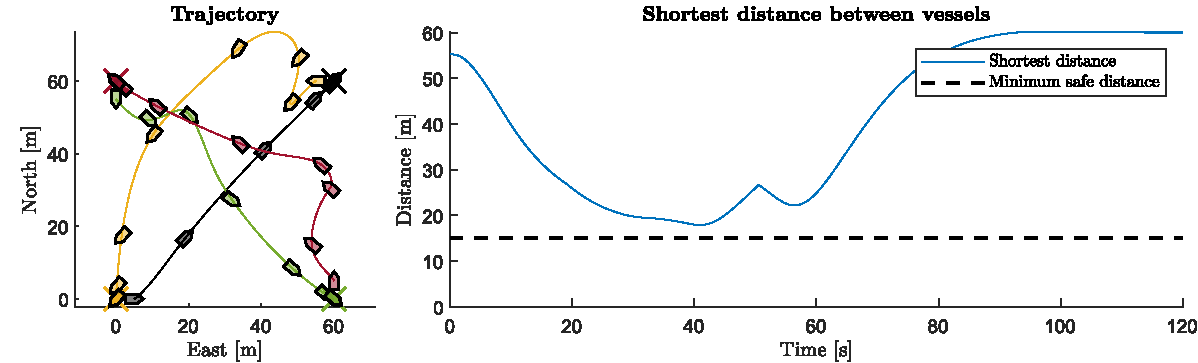
\includegraphics[width = \textwidth]{figures/ccta/milliAmpere_modified_uncontrolled.pdf}
        % This file was created by matlab2tikz.
%
%The latest updates can be retrieved from
%  http://www.mathworks.com/matlabcentral/fileexchange/22022-matlab2tikz-matlab2tikz
%where you can also make suggestions and rate matlab2tikz.
%
\definecolor{mycolor1}{rgb}{0.00000,0.44700,0.74100}%
\definecolor{mycolor2}{rgb}{0.85000,0.32500,0.09800}%
\definecolor{mycolor3}{rgb}{0.92900,0.69400,0.12500}%
\definecolor{mycolor4}{rgb}{0.49400,0.18400,0.55600}%

%
\begin{tikzpicture}

\begin{axis}[%
width=0.24\textwidth,
height=0.24\textwidth,
at={(0,0)},
scale only axis,
xmin=-10,
xmax=70,
xlabel style={font=\color{white!15!black}\small, yshift=1.5mm},
xlabel={East [m]},
ticklabel style={font=\small},
ymin=-4,
ymax=78,
ylabel style={font=\color{white!15!black}\small, yshift=-1.5mm},
ylabel={North [m]},
axis background/.style={fill=white},
title style={font=\bfseries, yshift=-2.5mm},
title={Trajectory},
xmajorgrids,
ymajorgrids,
]
\def\nboatplots{10}

\addplot [color=black, line width=0.8pt]
  table[]{milliAmpere_modified_uncontrolled-1.tsv};
\foreach \i in {1,...,\nboatplots}
  \addplot[area legend, draw=black, fill=black, fill opacity=0.75, line width=0.5pt]
  table[x=x\i, y=y\i]{milliAmpere_modified_uncontrolled-asv-1.tsv};

\addplot [color=mycolor2, line width=0.8pt]
  table[]{milliAmpere_modified_uncontrolled-2.tsv};
\foreach \i in {1,...,\nboatplots}
  \addplot[area legend, draw=black, fill=mycolor2, fill opacity=0.75, line width=0.5pt]
  table[x=x\i, y=y\i]{milliAmpere_modified_uncontrolled-asv-2.tsv};

\addplot [color=mycolor3, line width=0.8pt]
  table[]{milliAmpere_modified_uncontrolled-3.tsv};
\foreach \i in {1,...,\nboatplots}
  \addplot[area legend, draw=black, fill=mycolor3, fill opacity=0.75, line width=0.5pt]
  table[x=x\i, y=y\i]{milliAmpere_modified_uncontrolled-asv-3.tsv};

\addplot [color=mycolor4, line width=0.8pt]
  table[]{milliAmpere_modified_uncontrolled-4.tsv};
\foreach \i in {1,...,\nboatplots}
  \addplot[area legend, draw=black, fill=mycolor4, fill opacity=0.75, line width=0.5pt]
  table[x=x\i, y=y\i]{milliAmpere_modified_uncontrolled-asv-4.tsv};

\end{axis}

\begin{axis}[%
width=0.54\textwidth,
height=0.24\textwidth,
at={(0.35\textwidth,0)},
scale only axis,
xmin=0,
xmax=120,
xlabel style={font=\color{white!15!black}\small, yshift=1.5mm},
xlabel={Time [s]},
ymin=0,
ymax=61,
xmajorgrids,
ymajorgrids,
ticklabel style={font=\small},
ylabel style={font=\color{white!15!black}\small, yshift=-1.5mm},
ylabel={Distance [m]},
axis background/.style={fill=white},
title style={font=\bfseries, yshift=-2mm},
title={Shortest distance between vessels},
legend style={/tikz/column 2/.style={column sep=5pt,}, font=\small, at={(0.675,0.95)}, anchor=north east},
]
\addplot [color=mycolor1, line width=0.8pt]
  table[]{milliAmpere_modified_uncontrolled-5.tsv};
%\addlegendentry{Shortest distance}

\addplot [color=black, dashed, line width=1.5pt]
  table[]{milliAmpere_modified_uncontrolled-6.tsv};
%\addlegendentry{Minimum distance}

\end{axis}
\end{tikzpicture}%
        \caption{Algorithm \eqref{eq:ccta_combined_avoidance_allocation_modified} on four \emph{milliAmpere} vessels with one uncontrolled vessel}
        \vspace{0em}
    \end{subfigure}
    \begin{subfigure}{\linewidth}
        \centering
        %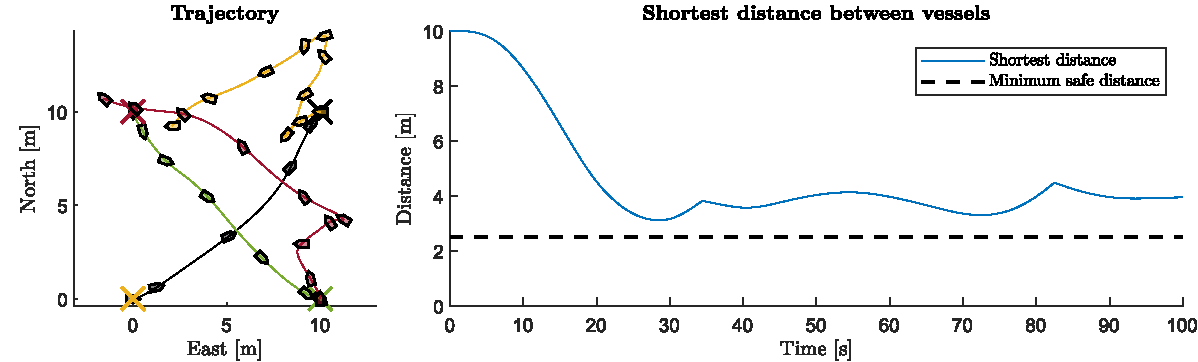
\includegraphics[width = \textwidth]{figures/ccta/drillship_modified_uncontrolled.pdf}
        % This file was created by matlab2tikz.
%
%The latest updates can be retrieved from
%  http://www.mathworks.com/matlabcentral/fileexchange/22022-matlab2tikz-matlab2tikz
%where you can also make suggestions and rate matlab2tikz.
%
\definecolor{mycolor1}{rgb}{0.00000,0.44700,0.74100}%
\definecolor{mycolor2}{rgb}{0.85000,0.32500,0.09800}%
\definecolor{mycolor3}{rgb}{0.92900,0.69400,0.12500}%
\definecolor{mycolor4}{rgb}{0.49400,0.18400,0.55600}%

%
\begin{tikzpicture}

\begin{axis}[%
width=0.24\textwidth,
height=0.24\textwidth,
at={(0,0)},
scale only axis,
xmin=-3,
xmax=13,
xlabel style={font=\color{white!15!black}\small, yshift=1.5mm},
xlabel={East [m]},
ticklabel style={font=\small},
ymin=-1,
ymax=15,
ylabel style={font=\color{white!15!black}\small, yshift=-3mm},
ylabel={North [m]},
axis background/.style={fill=white},
title style={font=\bfseries, yshift=-2.5mm},
title={Trajectory},
xmajorgrids,
ymajorgrids,
]
\def\nboatplots{10}

\addplot [color=black, line width=0.8pt]
  table[]{drillship_modified_uncontrolled-1.tsv};
\foreach \i in {1,...,\nboatplots}
  \addplot[area legend, draw=black, fill=black, fill opacity=0.75, line width=0.5pt]
  table[x=x\i, y=y\i]{drillship_modified_uncontrolled-asv-1.tsv};

\addplot [color=mycolor2, line width=0.8pt]
  table[]{drillship_modified_uncontrolled-2.tsv};
\foreach \i in {1,...,\nboatplots}
  \addplot[area legend, draw=black, fill=mycolor2, fill opacity=0.75, line width=0.5pt]
  table[x=x\i, y=y\i]{drillship_modified_uncontrolled-asv-2.tsv};

\addplot [color=mycolor3, line width=0.8pt]
  table[]{drillship_modified_uncontrolled-3.tsv};
\foreach \i in {1,...,\nboatplots}
  \addplot[area legend, draw=black, fill=mycolor3, fill opacity=0.75, line width=0.5pt]
  table[x=x\i, y=y\i]{drillship_modified_uncontrolled-asv-3.tsv};

\addplot [color=mycolor4, line width=0.8pt]
  table[]{drillship_modified_uncontrolled-4.tsv};
\foreach \i in {1,...,\nboatplots}
  \addplot[area legend, draw=black, fill=mycolor4, fill opacity=0.75, line width=0.5pt]
  table[x=x\i, y=y\i]{drillship_modified_uncontrolled-asv-4.tsv};

\end{axis}

\begin{axis}[%
width=0.55\textwidth,
height=0.24\textwidth,
at={(0.35\textwidth,0)},
scale only axis,
xmin=0,
xmax=100,
xlabel style={font=\color{white!15!black}\small, yshift=1.5mm},
xlabel={$t$ [s]},
ymin=0,
ymax=10.1,
xmajorgrids,
ymajorgrids,
ticklabel style={font=\small},
ylabel style={font=\color{white!15!black}\small, yshift=-1.75mm},
ylabel={Distance [m]},
axis background/.style={fill=white},
title style={font=\bfseries, yshift=-2mm},
title={Shortest distance between vessels},
legend style={/tikz/column 2/.style={column sep=5pt,}, font=\small, at={(0.98,0.97)}, anchor=north east},
]
\addplot [color=mycolor1, line width=0.8pt]
  table[]{drillship_modified_uncontrolled-5.tsv};
\addlegendentry{Shortest distance}

\addplot [color=black, dashed, line width=1.5pt]
  table[]{drillship_modified_uncontrolled-6.tsv};
\addlegendentry{Minimum distance}

\end{axis}
\end{tikzpicture}%
        \caption{Algorithm \eqref{eq:ccta_combined_avoidance_allocation_modified} on four drillships with one uncontrolled vessel}
        \label{fig:ccta_drillship_unc}
        \vspace{-1.5mm}
    \end{subfigure}
    \caption{Simulations of the modified control allocation algorithm \eqref{eq:ccta_combined_avoidance_allocation_modified} with one uncontrolled vessel (plotted in black)}
    \label{fig:ccta_uncontrolled}
    \vspace{-6mm}
\end{figure*}

\section{Conclusions}
\label{sec:ccta_conclusion}
In this chapter, we have proposed a method for integrating a \gls{colav} scheme into control allocation through control barrier functions.
We have demonstrated its effectiveness on two models of ASVs, where it significantly improved the safety.
The proposed method can be readily implemented on vehicles that already use optimization-based control allocation by simply including the constraints given by the control barrier functions in the optimization.

Finding a systematic method for choosing the parameter values that guarantee safety for a given vehicle model is a topic for future work.
